\documentclass[a4paper,12pt]{article}

\usepackage{amsmath,amssymb,amsthm,tikz}
\usetikzlibrary{calc,arrows.meta}
\usepackage[margin=20mm]{geometry}
\usepackage{hyperref}

\setlength{\parindent}{0pt}
\setlength{\columnsep}{1cm}

\begin{document}

\twocolumn

\thispagestyle{empty}

\begin{center}
{\Large Assignment 11}\\
{\Large Published on 2020-12-05,}\\
{\em Estimated Time: 30 minutes,}\\
{\em Max.grade 10\textperthousand} 
\end{center}


\section{Introduction}

If you know how to do topological sorting using 
the DFS traversal (recording their 
discovery and final visit times), you can immediately 
start with the items in Section 2.
You can also read an inspirational slide deck on TOpological Sorting 
from University of California, Davis:\\
\url{https://www.cs.ucdavis.edu/~bai/ECS122A/Notes/DFSapps.pdf}. 
Or (Goodrich2011, p.633), 
{\em Section 13.4.3 Directed Acyclic Graphs}.


In the example below we show the following: 
\begin{itemize}
\item Draw the visual representation from its adjancency list
representation.
\item Add two more edges to the graph. 
\item Run the DFS to check, if it is still a DAG (directed acyclic graph). 
We do that DFS in a repeatable order (always pick the lexicographically smallest
vertex, if there is a choice). 
\item Use the DFS visiting order (``final'' timestamp) to 
create the topological sorting.
\end{itemize}


\subsection{Sample DAG}

Mr.\ Bunbury dresses every morning according to
certain rules: He always puts on his Trousers
after Underpants, his Sweater after his Belt. 
He also puts on his Face-mask after the Sweater 
(otherwise it would displace the Face-mask 
as it is pulled over the head), 
glasses are put on after the Face-mask, 
since otherwise they get foggy, and so on.

\begin{figure}[!htb]
\center{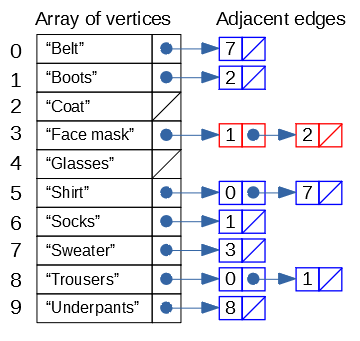
\includegraphics[width=3in]{assignment11-topological-sort/clothing-adjacent.png}}
\caption{\label{fig:clothing-adjacent} Adjacency List Representation}
\end{figure}

All the rules are shown in graph $G$ Figure~\ref{fig:clothing-adjacent}
(it is also the adjecency list representation; 
it shows all the before-after binary relationships). Square cells
that are crossed diagonally show null-pointers (i.e.\ they denote 
where the adjacency lists end). 
Mr.\ Bunbury has figured how he can get dressed according to these rules.
To make it even more intuitive, he made a visual 
representation of the rules as in Figure~\ref{fig:clothing-dag}.

Somebody tells Mr.\ Bunbury that his Coat and Boots may be contaminated 
with viruses, but hands should be clean as he applies the Face-mask 
(this adds two red arrows to the diagram in Figure~\ref{fig:clothing-dag}).
At this point Mr.\ Bunbury needs advice \textendash{} one 
feasible way to get dressed 
by {\em topologically sorting} the clothing items
(or an evidence of a contradiction: a loop of arrows that prove 
that the updated graph is not a 
{\em Directed Acyclic Graph} anymore and it cannot be sorted).

\begin{figure}[!htb]
\center{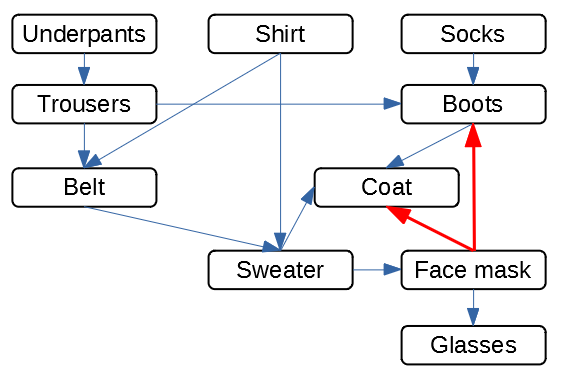
\includegraphics[width=3in]{assignment11-topological-sort/clothing-dag.png}}
\caption{\label{fig:clothing-dag} Graph $G$ visualized}
\end{figure}



\subsection{DFS Traversal Example}

The Depth-First-Search traversal is described by a 
recursive algorithm having this pseudocode:

$$\begin{array}{rl}
 & \text{\sc DFS}(G)\\
1 & \text{\bf for each}\;\text{vertex}\;u \in G.V:\\
2 & \hspace{.5cm} u.\text{\em color} = \text{\sc white}\\
3 & \hspace{.5cm} u.\text{\em parent} = \text{\sc nil}\\
4 & \text{\em time} = 0\\
5 & \text{\bf for each}\;\text{vertex}\;u \in G.V:\\
6 & \hspace{.5cm} \text{\bf if}\;u.\text{\em color} == \text{\sc white}:\\
7 & \hspace{1cm} \text{\sc DFS\textunderscore{}Visit}(G,u)\\
\end{array}$$

The loop on Line 5 (see the pseudocode of
$\text{\sc DFS}(G)$ above) visits vertices $u \in G.V$ 
in the lexicographic order. (It may also happen that 
$\text{\sc DFS\textunderscore{}Visit}(G,u)$ is invoked just once, if
a single DFS call is enough to visit every vertex and to turn it black.

Here is the code of $\text{\sc DFS\textunderscore{}Visit}(G,u)$ (the DFS-visit 
for vertex $u \in G.V$). Please pay attention to the two parameters 
$\text{\em u.d}$ (discovery time \textendash{} when the DFS 
traversal enters $u$ for the first time) and $\text{\em u.d}$ (finish time \textendash{}
when the DFS traversal leaves $u$ forever, since $u$ is visited along with all 
its freshly discovered child vertices). 

$$\begin{array}{rl}
  & \text{\sc DFS\textunderscore{}Visit}(G,u)\\
1 & \text{\em time} = \text{\em time} + 1 \\
  & \textcolor{teal}{\small \text{\em (white vertex $u$ was just discovered)}}\\
2 & u.d = \text{\em time}\\
3 & u.\text{\em color} = \text{\sc gray}\\
  & \textcolor{teal}{\small \text{\em (explore $(u,v_1)$, $(u,v_2)$, $\ldots$)}}\\
4 & \text{\bf for each}\;v \in G.Adj[u]: \\ 
5 & \hspace{0.5cm} \text{\bf if}\;v.\text{\em color} == \text{\sc white}:\\
6 & \hspace{1cm} v.\text{\em parent} = u\\
7 & \hspace{1cm} \text{\sc DFS\textunderscore{}Visit}(G,u)\\
  & \textcolor{teal}{\small \text{\em (vertex u now fully processed)}}\\
8 & u.\text{\em color} = \text{\sc black}\\
9 & \text{\em time} = \text{\em time} + 1\\
10 & u.f = \text{\em time}\\
\end{array}$$


Once again, we assume that the white neighbors of $u$ (for example, 
$v_1$, $v_2$) are visited in their lexicographic order. 
These assumptions make DFS traversal repeatable (without such assumption there 
are typically multiple ways how to do DFS-style visits). 

Let us run this DFS pseudocode on the clothing graph. 
We start by visiting the vertex ``Belt'' (as it is alphabetically first), 
so its discovery time $u.d = 1$. After that we visit all its neighbors (in their 
alphabetical order, if there are several). 
When we finish processing ``Belt'', we find the next vertex
(alphabetically first among those unvisited or having color {\sc white}), and so on. 
The result of these activities is shown in Figure~\ref{fig:clothing-dfs}
(each vertex in $G$ has a green pair $(d/f)$ that shows the discovery/finish 
time). 

\begin{figure}[!htb]
\center{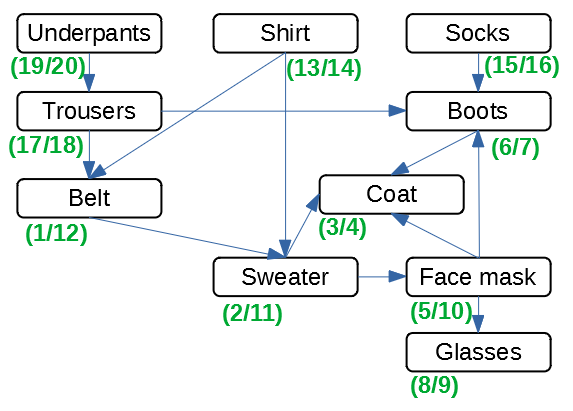
\includegraphics[width=3in]{assignment11-topological-sort/clothing-dfs.png}}
\caption{\label{fig:clothing-dfs} Graph $G$ with DFS discovery/finish}
\end{figure}



\subsection{Getting Topological Sorting}

$$\begin{array}{rl}
  & \text{\sc Topological\textunderscore{}Sort}(G)\\
  & \textcolor{teal}{\small \text{\em (result accumulates in reverse order)}}\\
1 & S = \text{\sc Stack.Empty()}\\
2 & \text{call}\;\text{\sc DFS}(G)\\
3 & \text{\bf for each}\;u \in G.V:\\ 
4 & \hspace{0.5cm} \text{as soon as $u.f$ (finish time) is assigned}:\\
5 & \hspace{0.5cm} S.\text{\em push}(u)\\
6 & \text{\bf return}\;S\\
\end{array}$$

We can look at Figure~\ref{fig:clothing-dfs} and list all the nodes in the 
reverse order of their finish times (their values are $20,18,16,14,12,11,10,9,7,4$), 
we would get the following topological order (one feasible way how 
Mr.\ Bunbury can dress himself). For every clothing item we
also specify the time value when that vertex was finished (painted black).

\begin{quote}
(20) Underpants; (18) Trousers;\\
(16) Socks; (14) Shirt;\\
(12) Belt; (11) Sweater;\\
(10) Face mask; (9) Glasses;\\
(7) Boots; (4) Coat. 
\end{quote}

The sequence shows that DFS (and the formal rule that always
picks the lexicographically smallest item) causes a reasonable 
advice to get dressed.



\subsection{Graphs that are Not DAGs}

Topological sorting is not always doable \textendash{} if there 
is any loop in the graph, it is no longer a DAG 
(a directed acyclical graph). 
During the DFS traversal it is possible to verify, 
if a graph is a DAG or not. 

Let us remember, how all directed edges fall into 4 categories as we 
perform DFS: 
\begin{description}
\item[Tree/Discovery edges] \hfill \\
All the edges $(u,v)$ visited by DFS as the depth-first forest is built (see Line 4 
in pseudocode $\text{\sc DFS\textunderscore{}Visit}(G,u)$). 
\item[Back edges] \hfill \\ 
Edges connecting a vertex $u$ with its ancestor $v$ in some DFS tree.
(If a cyclical graph contains a loop $(v,v)$ from a vertex to itself, 
it is considered a back edge as well.)
\item[Forward edges] \hfill\\
Non-tree edges $(u,v)$ connecting $u$ to a descendant $v$ in some DFS tree. 
\item[Cross edges] \hfill\\
All the other edges \textendash{} a cross edge connects a vertex to a vertex 
that is neither its ancestor nor its descendent
\end{description}




{\bf Statement.} A graph is a DAG iff there is no 
back edge: all edges during the DFS traversal are either
discovery edges, forward edges or cross edges. 

{\bf Example.} Consider the graph in Figure~\ref{fig:cyclical-graph}. 
It has a back-edge $(D,A)$ which completes a cycle 
(in this example it is made from $3$ edges: $(A,B)$, $(B,D)$, $(D,A)$)

\begin{figure}[!htb]
\center{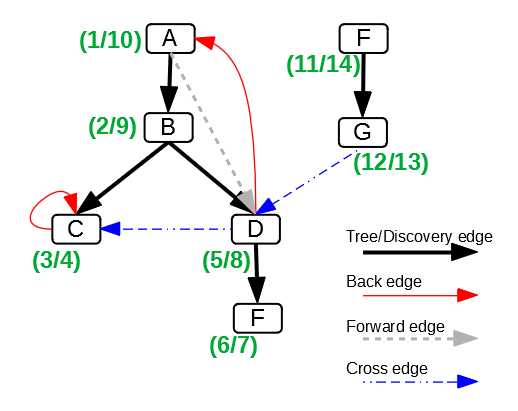
\includegraphics[width=3in]{assignment11-topological-sort/cyclical-graph.png}}
\caption{\label{fig:cyclical-graph} A graph with a cycle}
\end{figure}


To identify directed graphs that are not acyclical, 
modify Line 4 in the pseudocode of\\
$\text{\sc DFS\textunderscore{}Visit}(G,u)$: 
Before adding the new discovery/tree edge $(u,v)$, check, 
if $u$ has any neighbor $v^{\ast}$ that currently has color {\sc gray}; 
this would mean that $v^{\ast}$ is an ancestor of $u$ and 
$(u,v^{\ast})$ is a back-edge, which is forbidden.
(Even in case when $v^{\ast} = u$, and the edge $(u,v^{\ast})$ is 
a loop to itself, the check would reveal that $u$ has color {\sc gray}.)




\section{Problem}

We start with the graph shown in Figure~\ref{fig:problem-adjacent}.

\begin{figure}[!htb]
\center{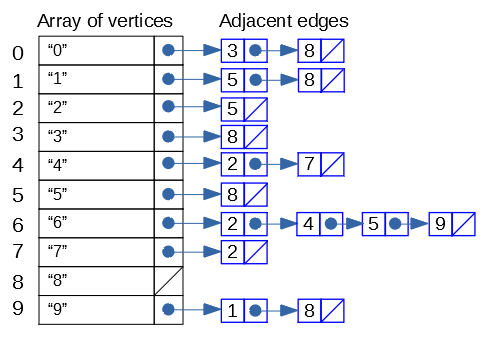
\includegraphics[width=3in]{assignment11-topological-sort/problem-adjacent.png}}
\caption{\label{fig:problem-adjacent} Adjacency list representation}
\end{figure}

\vspace{10pt}
{\bf (A)} Draw the visual representation of the graph, 
each vertex is a circle (with string values {\tt "0"} to {\tt "9"})
inside. If there is a directed edge from one vertex to another, 
draw it as an arrow.\\
(Figures \ref{fig:clothing-adjacent} and \ref{fig:clothing-dag} show
how this transformation was made for the clothing graph.)

\vspace{10pt}
{\bf (B)} Compute the following $4$ numbers from $a,b,c$ (your last 
Student ID numbers): 
$$\left\{ \begin{array}{l}
T = 3 \cdot ((a+b)\;\text{mod}\;4)\\
U = 3 \cdot ((b+c)\;\text{mod}\;3)+1\\
V = 3 \cdot ((c+a)\;\text{mod}\;3)+1\\
W = 3 \cdot ((a+b+c)\;\text{mod}\;3)+2\\
\end{array} \right.$$

By $(x\;\text{mod}\;y)$ we denote the remainder as $x$ is divided by $y$. 
Add to the original graph two new directed edges $(T,U)$ and $(V,W)$. 
(For example, if $T = 5$ and $U = 7$, then there should be an arrow from 
vertex {\tt "5"} to vertext {\tt "7"}. If such an edge already exists, do 
not add anything.)

Draw the new graph; show the newly added edges in bold or colored differently.

\vspace{10pt}
{\bf (C)} Run the DFS traversal algorithm on the graph just obtained in (B), mark each vertex 
with the pair of numbers {\tt d/f}, where the first number {\tt d} is the 
discovery time, and the second number {\tt f} is the finishing time. 
(You will use all the numbers from $1$ to $20$: every number will be used
exactly once.) It should take exactly $20$ steps to do DFS enters/exits in 
a directed graph with $10$ vertices.

If there are multiple ways how to pick a vertex to visit next, always
pick the vertex with the smallest number. (Otherwise your results cannot be
properly verified.)

\vspace{10pt}
{\bf (D)} If the graph you got in (B) after adding new edges is not a DAG anymore, 
please say so in your answer; indicate what vertex you visited as you discovered 
that a back edge exists. And also show which is the cycle.

If the graph is a DAG, produce a topological sorting of its vertices
(the algorithm is explained in Section 1.4 above). 

\vspace{10pt}
{\em Note.} Your solution should contain two directed graphs ((A) and (B)), one
directed graph with vertices anotated with {\tt d/f} (in (C)) and 
EITHER information on the back edge+cycle OR topological sorting of the vertices.


\end{document}

